% ----------------------------------------------------------------------------------------------------------
% Praeambel
% ----------------------------------------------------------------------------------------------------------
\documentclass[fontsize=12pt,%
paper=a4,%
DIV=classic,%
%BCOR=10mm,%
twoside=true,%
headings=openany,%
parskip=half+,%
pagesize=auto,%
numbers=noenddot,%
headsepline=true,%
toc=listof,%
toc=bibliography%
]{scrreprt}

% PDF-Kompression
\pdfminorversion=5
\pdfobjcompresslevel=1

% Schriften
%\usepackage{mathpazo,tgpagella}
%\usepackage{libertine}
%\usepackage{fourier}
\usepackage{lmodern}

% Allgemeines
\usepackage{amsmath,amssymb} % Mathesachen
\usepackage[T1]{fontenc} % Ligaturen, richtige Umlaute im PDF
\usepackage[utf8]{inputenc}% UTF8-Kodierung für Umlaute usw

\usepackage{siunitx}
\usepackage{scrlayer-scrpage} 
\pagestyle{scrheadings}

%\usepackage{setspace}
%\onehalfspacing 

% Schriften-Größen
\setkomafont{chapter}{\Huge\rmfamily}
\setkomafont{section}{\Large\rmfamily}
\setkomafont{subsection}{\large\rmfamily}
\setkomafont{subsubsection}{\large\rmfamily}
\setkomafont{chapterentry}{\large\rmfamily} % Überschrift der Ebene in Inhaltsverzeichnis
\setkomafont{descriptionlabel}{\bfseries\rmfamily} % für description Umgebungen
\setkomafont{captionlabel}{\small\bfseries}
\setkomafont{caption}{\small}

% Sprache: Deutsch
\usepackage[autostyle,babel,german=guillemets,style=german]{csquotes}
\usepackage[USenglish,ngerman]{babel} 
\selectlanguage{ngerman}
% PDF
\usepackage[ngerman,%
pdfauthor={B. Ternes, J. Feldkamp},%
pdftitle={Modellbasierte Implementierung einer Vektorregelung für Synchronmaschinen},%
colorlinks=true,linkcolor=blue,citecolor=blue,filecolor=magenta,urlcolor=blue%
]{hyperref}

% BibLaTeX
\usepackage[backend=biber,%
 style=authoryear,%
 bibstyle=authoryear,%
 citestyle=authoryear,%
 % autocite=inline,%
 sorting=anyt,%
 sortcites=true,%
 hyperref=auto,%
 maxnames=3,%
 minnames=1,%
]{biblatex}

\bibliography{bibo.bib}

\setlength{\bibitemsep}{1em}
\DefineBibliographyStrings{ngerman}{andothers = {u.\,a.},}

\usepackage[final]{microtype} % mikrotypographische Optimierungen
\usepackage{url}
\usepackage{pdflscape} % einzelne Seiten drehen können

% Tabellen
\usepackage{multirow} % Tabellen-Zellen über mehrere Zeilen
\usepackage{multicol} % mehre Spalten auf eine Seite
%\usepackage{tabularx} % Für Tabellen mit vorgegeben Größen
\usepackage{booktabs}
\usepackage{longtable} % Tabellen über mehrere Seiten
\usepackage{array}

%  Bibliographie
%\usepackage{bibgerm} % Umlaute in BibTeX

% Tabellen
\usepackage{multirow} % Tabellen-Zellen über mehrere Zeilen
\usepackage{multicol} % mehre Spalten auf eine Seite
\usepackage{tabularx} % Für Tabellen mit vorgegeben Größen
\usepackage{array}
\usepackage{float}

% Bilder
\usepackage{graphicx}
\usepackage{color}
\graphicspath{{_Bilder/}}

\DeclareGraphicsExtensions{.pdf,.png,.jpg}
\usepackage{subfigure}
\newcommand{\subfigureautorefname}{\figurename}
\usepackage[all]{hypcap}

% Bildunterschrift
\setcapindent{0em}
\setcapwidth[c]{0.9\textwidth}
\setlength{\abovecaptionskip}{0.2cm}

% Quellcode
\usepackage{listings}
\definecolor{grau}{gray}{0.25}
\lstset{
	extendedchars=true,
	basicstyle=\tiny\ttfamily,
	%basicstyle=\footnotesize\ttfamily,
	tabsize=2,
	keywordstyle=\textbf,
	commentstyle=\color{grau},
	stringstyle=\textit,
	numbers=left,
	numberstyle=\tiny,
	% für schönen Zeilenumbruch
	breakautoindent  = true,
	breakindent      = 2em,
	breaklines       = true,
	postbreak        = ,
	prebreak         = \raisebox{-.8ex}[0ex][0ex]{\Righttorque},
}

% linksbündige Fußboten
\deffootnote{1.5em}{1em}{\makebox[1.5em][l]{\thefootnotemark}}

\usepackage[right=3cm,left=2cm]{geometry}

%\typearea{14} % typearea berechnet einen sinnvollen Satzspiegel (das heißt die Seitenränder) siehe auch http://www.ctan.org/pkg/typearea. Diese Berechnung befindet sich am Schluss, damit die Einstellungen oben berücksichtigt werden
% für autoref von Gleichungen in itemize-Umgebungen
\makeatletter
\newcommand{\saved@equation}{}
\let\saved@equation\equation
\def\equation{\@hyper@itemfalse\saved@equation}
\makeatother 

\usepackage[framemethod=TikZ]{mdframed}
\usepackage{xcolor}

\definecolor{light-gray}{gray}{0.85}

\newmdenv[%
    backgroundcolor=light-gray,
    linecolor=light-gray,
    outerlinewidth=2pt,
    roundcorner=2mm,
    skipabove=\baselineskip,
    skipbelow=\baselineskip,
]{shaded}
\newcommand{\mat}[1]{
      {\textbf{#1}}
}

\newcommand{\todo}[1]{
      {\colorbox{red}{ TODO: #1 }}
}

\newcommand{\todotext}[1]{
      {\color{red} TODO: #1} \normalfont
}

\newcommand{\info}[1]{
      {\colorbox{blue}{ (INFO: #1)}}
}

% Hinweis auf Programme in Datei
\newcommand{\datei}[1]{
      {\ttfamily{#1}}
}
\newcommand{\code}[1]{
      {\ttfamily{#1}}
}
% bild mit defnierter Breite einfügen
\newcommand{\bild}[4]{
  \begin{figure}[!hbt]
    \centering
      \vspace{1ex}
      \includegraphics[width=#2]{images/#1}
      \caption[#4]{\label{img.#1} #3}
    \vspace{1ex}
  \end{figure}
}
% bild mit eigener Breite
\newcommand{\bilda}[3]{
  \begin{figure}[!hbt]
    \centering
      \vspace{1ex}
      \includegraphics{images/#1}
      \caption[#3]{\label{img.#1} #2}
      \vspace{1ex}
  \end{figure}
}


% Bild todo
\newcommand{\bildt}[2]{
  \begin{figure}[!hbt]
    \begin{center}
      \vspace{2ex}
	      \includegraphics[width=6cm]{images/todobild}
      %\caption{\label{#1} \color{red}{ TODO: #2}}
      \caption{\label{#1} \todotext{#2}}
      %{\caption{\label{#1} {\todo{#2}}}}
      \vspace{2ex}
    \end{center}
  \end{figure}
}

\usepackage{xspace} 
\newcommand{\AdV}{Anm.\ d.\ Verf.\@\xspace}
\newcommand{\bzw}{bzw.\@\xspace}
\newcommand{\etc}{etc.\@\xspace}
\newcommand{\bspw}{bspw.\@\xspace}
\newcommand{\bzgl}{bzgl.\@\xspace}
\newcommand{\ea}{et\,al.\@\xspace}
\newcommand{\etal}{et\,al.\@\xspace} 
\newcommand{\latex}{\LaTeX\@\xspace}
\newcommand{\insb}{insbesondere}
\newcommand{\dH}{d.\,h.\@\xspace}
\newcommand{\ggf}{ggf.\@\xspace}
\newcommand{\ggfs}{ggfs.\@\xspace}
\newcommand{\idr}{i.\,d.\,R.\@\xspace}
\newcommand{\ivm}{i.\,V.\,m.\@\xspace}
\newcommand{\ieS}{i.\,e.\,S.\@\xspace}
\newcommand{\is}{i.\,S.\@\xspace}
\newcommand{\iwS}{i.\,w.\,S.\@\xspace}
\newcommand{\oae}{o.\,{\"a}.\@\xspace}
\newcommand{\og}{o.\,g.\@\xspace}
\newcommand{\ua}{u.\,a.\@\xspace}
\newcommand{\uae}{u.\,{\"a}.\@\xspace}
\newcommand{\usw}{usw.\@\xspace}
\newcommand{\uU}{u.\,U.\@\xspace}
\newcommand{\uvm}{u.\,v.\,m.\@\xspace}
\newcommand{\va}{v.\,a.\@\xspace}
\newcommand{\zB}{\mbox{z.\,B.}\@\xspace}
\newcommand{\zt}{z.\,T.\@\xspace}
\newcommand{\vglzb}{vgl.\,z.\,B.\@\xspace}
\newcommand{\vgl}{vgl.\@\xspace}
\newcommand{\sog}{sog.\@\xspace}
\newcommand{\so}{s.\,o.\@\xspace}
\newcommand{\msc}{M.\,Sc.\@\xspace}
\newcommand{\bsc}{B.\,Sc.\@\xspace} 

\begin{document}
\pagenumbering{Roman}
\pagestyle{empty}

% ----------------------------------------------------------------------------------------------------------
% Titelseite
% ----------------------------------------------------------------------------------------------------------
\clearscrheadings\clearscrplain

\begin{center}
	\begin{minipage}{7cm}
	\textsc{Fachbereich Elektrotechnik\\
	und Informatik}\\
	\\
	Institut für Systemtechnik
	\end{minipage}
	\hfill
	\begin{minipage}{7cm}
	
\includegraphics[width=\textwidth]{bo}\\
	\end{minipage}
	
	\vspace*{4cm}
	
	\Huge
	\textbf{Projektarbeit}\\
	\vspace*{0.5cm}
	\large
	über das Thema\\
	\vspace*{1cm}
	\Huge
	\textbf{Auslegung eines parametriesierten Modells einer vektorgeregelten anisotropen Synchronmaschine}\\
	\vspace*{2cm}
	\vfill
	\normalsize
	\newcolumntype{x}[1]{>{\raggedleft\arraybackslash\hspace{0pt}}p{#1}}
	\begin{tabular}{x{6cm}p{7.5cm}}
		\rule{0mm}{5ex}\textbf{Autoren:} & Benjamin Ternes\newline benjamin.ternes@fernuni-hagen.de\newline Matrikelnummer: 014102076 \\
		\rule{0mm}{5ex}                & Jan Feldkamp\newline jan.feldkamp@hs-bochum.de \newline Matrikelnummer: XXXXXXXXXX\\ 
		\rule{0mm}{5ex}\textbf{Prüfer:} & Prof. Dr.-Ing. A. Bergmann \\ 
		\rule{0mm}{5ex}\textbf{Abgabedatum:} & \today \\ 
	\end{tabular} 
\end{center}
\clearpage

\pagestyle{scrheadings}
\ohead[]{\pagemark}
\ihead[]{\headmark}
\ifoot[]{}
\automark[chapter]{chapter}
\automark*[section]{}
\renewcommand*{\chapterpagestyle}{scrheadings}
% ----------------------------------------------------------------------------------------------------------
% Verzeichnisse
% ----------------------------------------------------------------------------------------------------------
\tableofcontents
\listoffigures
\listoftables

\chapter*{Symbolverzeichnis}\label{s.sym}
\addcontentsline{toc}{chapter}{Symbolverzeichnis}
\markboth{Symbolverzeichnis}{Symbolverzeichnis}
% ----------------------------------------------------------------------------------------------------------
% Symbolliste
% ----------------------------------------------------------------------------------------------------------
\section*{Allgemeine Symbole}\label{s.sym.alg}
\begin{flushleft}\begin{tabularx}{\textwidth}{l l X}
Symbol & Bedeutung	& Einheit\\
\\
\hline
\\ 
$I$	& elektrische Stromstärke	&	$A$ \\
$\Theta$	&	elektrische Durchflutung 	&	$A$	\\
$A$			&	elektrischer Strombelag  	&  	$A/m$\\ 
$J$			&	elektrische Stromdichte		&	$A/m^2$ \\	
$H$			&	magnetische Feldstärke		&	$A/m$\\
$\mu_0$		&	magnetische Feldkonstante	&	$Vs/Am$\\
$\mu_r$		&	relative Permeabilität		&	\\
$B$			&	magnetische Flussdichte		&	$T = Vs/m^2$ \\
$\Phi$		&	magnetischer Fluss			&	$Vs$ \\
$\Psi$		&	verketteter Fluss			&	$Vs$ \\
$L, M$		&	Induktivitäten				&	$H = Vs/A$\\
$U$			&	elektrische Spannung		&	$V$ \\
$V$			&	magnetisches Vektorpotenzial&	$Vs/m$\\
$V_m$		&	magnetische Spannung		&	$A$
\end{tabularx}\end{flushleft}
% ----------------------------------------------------------------------------------------------------------
% Einleitung
% ----------------------------------------------------------------------------------------------------------
\pagenumbering{arabic}
%\input{Einleitung}
% ----------------------------------------------------------------------------------------------------------
% Kapitel
% ----------------------------------------------------------------------------------------------------------
\cleardoublepage
% -*- coding: utf-8 -*-
% !TEX encoding = UTF-8 Unicode
% !TEX root =  main.tex

\chapter{Theoretische und begriffliche Grundlagen}\label{cha:grundlagen}

Um auf die Regelung einer anisotropen Synchronmaschine einzugehen, werden im folgenden einige Grundlagen erörtert.

\section{Dreiphasensystem}\label{sec:dreiphasensystem}

\begin{figure}[h]
\centering
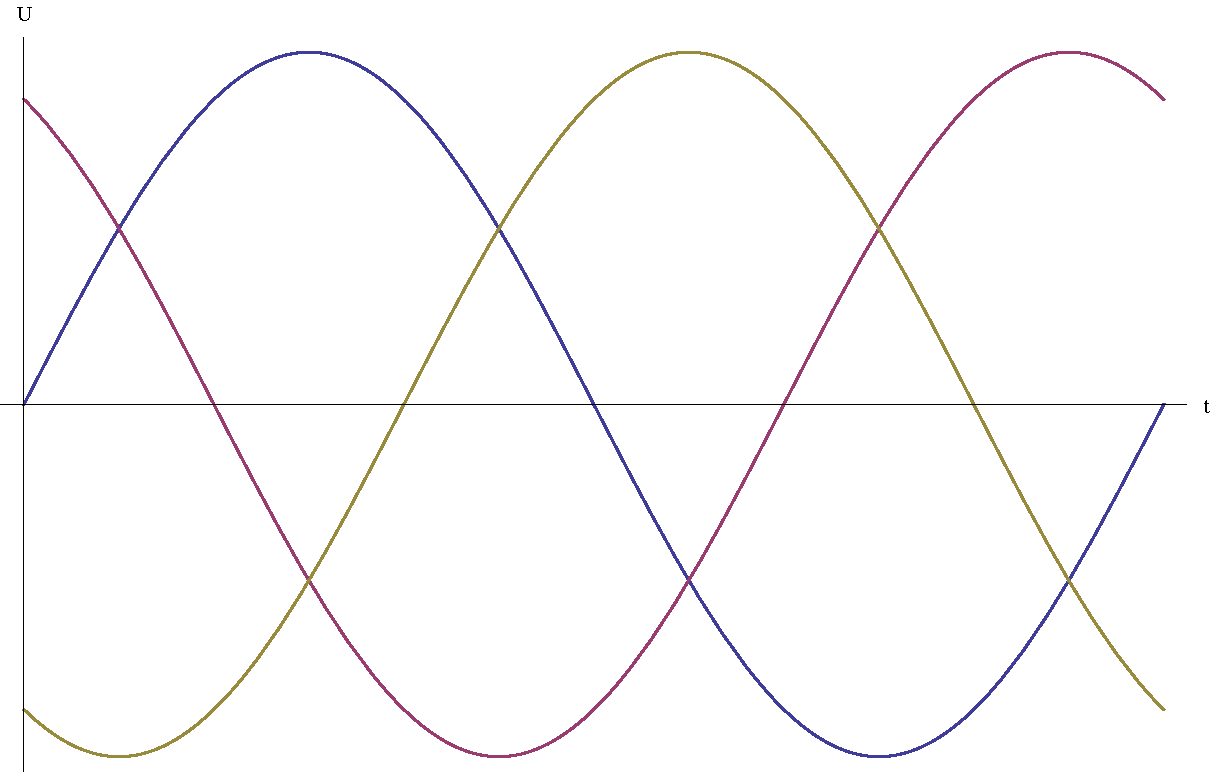
\includegraphics[width=0.5\textwidth]{dreiphasensystem.pdf}
\label{fig:dreiphasensystem}
\caption{Darstellung des Dreiphasensystem mit \textsc{Mathematica}.}
\end{figure}

\section{Einführung Magnetfelder}\label{sec:magnetfelder}

\subsection{Strombelag}\label{sec:strombelag}

Die zeitliche und örtliche Änderung von Magnetfeldern in elektrischen Maschinen wird bestimmt durch die Anordnung stromdurchflossener Leiter und die Art der Speisung \parencite[S.~199]{hofmann2013}.
Die räumliche Verteilung des Stromes wird durch den Strombelag wiedergegeben.
Wenn die Oberfläche eines ferromagnetischen Körpers einen Strombelag $A$ führt, d.\ h.\ wenn eine flächenhafte Strömung vorliegt, liefert das Durchflutungsgesetz

\begin{align}
\oint_{s}{\vec{H}d\vec{s}} = w\cdot I = \Theta \label{durchflutungsgesetz}
\end{align}

$Hds=Ads$, d.\ h.\ $H = A$ bzw.\ $B = \mu A$.
Folgernd existieren neben den Normalkomponenten, $B_n$ und $H_n$ die Tangentialkomponenten $H_t$ und $B_t$ der Feldgrößen.
Die Feldlinien treten nicht mehr senkrecht aus der Randkurve aus, sondern unter einem Winkel $\alpha$.

\begin{align}
\alpha = \arctan(\frac{B_n}{\mu A}) \label{strombelagwinkel}
\end{align}

Der Strombelag wird über dem Umlauf einer Spule bzw.\ Spulengruppe angegeben.

\begin{align}
\Theta(x) = - \int_{x_0}^{x} A(x)dx \label{durchflutung}
\end{align}

damit erhält man durch Differentation den Strombelag $A$

\begin{align}
A(x) = -\partial_x \Theta(x) \label{Strombelag}
\end{align}

mit

\begin{align}
\Theta(x) = \hat{\Theta}(x)\cdot \cos(\frac{\pi}{\tau_p}(x-x_\mu)) \label{adurchflutung}
\end{align}

Nach \ref{durchflutung} ist offensichtlich, dass eine sinusförmige Durchflutungsverteilung nur dann entstehen kann, wenn der Ankerstrombelag ebenfalls sinusförmig, aber um eine Polteilung versetzt ist \parencite[S.~247]{mullerI2005}.

%\begin{figure}[h]
%\centering
%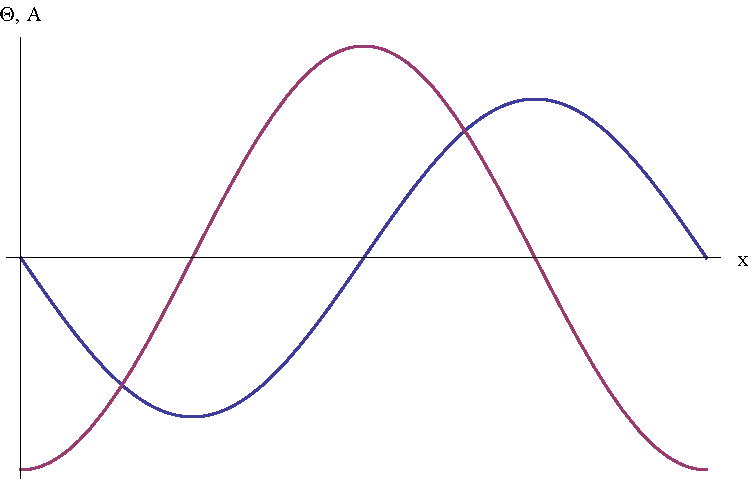
\includegraphics[width=0.5\textwidth]{strombelag.pdf}
%\label{fig:strombelag}
%\caption{Darstellung des sinusförmigen Verlaufs des Strombelags über dem Umlauf.}
%\end{figure}

\section{Allgemeine Grundlagen der Drehstrommaschinen}\label{sec:drehstrommaschinen}

Die Synchron- und Asynchronmaschine besitzen im Ständer denselben Aufbau und erfordern zur Darstellung ihres Verhaltens eine Reihe gleicher physikalischer Begriffe.
Es ist zweckmäßig die Grundlagen der Synchronmaschine in einem eigenen Kapitel zu behandeln.
Dies gilt \insb für den Aufbau der Drehstromwicklungen sowie die Grundlagen zu Beschreibung von umlaufenden Durchflutungen und deren Felder.

\subsection{Drehstromwicklungen}

Der prinzipielle Aufbau einer Drehstromwicklung lässt sich anhand aus den Anforderungen zur Erzeugung einer dreiphasigen Wechselspannung erläutern.
Eine solche Drehspannung erhält man mit einer Anordnung nach \autoref{fig:drehstromwicklung}.
Ein aus Dynamoblechen geschichtetes Ständerblechpacket enthält in Nuten am Bohrungsumfang gleichmäßig verteilte Leiter, die zu drei räumlich verteilten Wicklungssträngen zusammengeschaltet werden \autocite[S.~141]{fischer2009}.
Der Läufer erzeugt ein Gleichfeld, das eine sinusförmige Feldverteilung längst des Luftspaltes aufbaut.
Hat der Läufer eine konstante Drehzahl, so induziert das Feld in den einzelnen Spulen zeitlich sinusförmige Spannungen, die sich innerhalb eines Wicklungsstranges zu einem Wert addieren.
Die Berechnung der Induktion kann über die Allgemeine Beziehung

\begin{align}
u_q = B\cdot l \cdot v
\end{align}

erfolgen.
Sei $d_1$ der Bohrungdurchmesser des Ständerblechpaketes einer $2p$-poligen Maschine, so bezeichnet man den Umfangsanteil

\begin{align}
\tau_p = \frac{d_1 \cdot \pi}{2p}
\end{align}

wieder als Polteilung.
Die Polteilung entspricht der Länder einer Halbwelle der sinusförmigen Flussdichteverteilung im Luftspalt (enspricht einem elektrischen Winkel von $\omega t = 180^{\circ}$.
Bei einer zweipoligen Maschine mit $p=1$ stimmen somit der räumlich mechanische und der elektrische Winkel überein, allgemein gilt die Beziehung \autocite[S.141f.]{fischer2009}

\begin{align}
\gamma_{el} = p\cdot \gamma_{mech}
\end{align}



\begin{figure}[!htb]
\centering
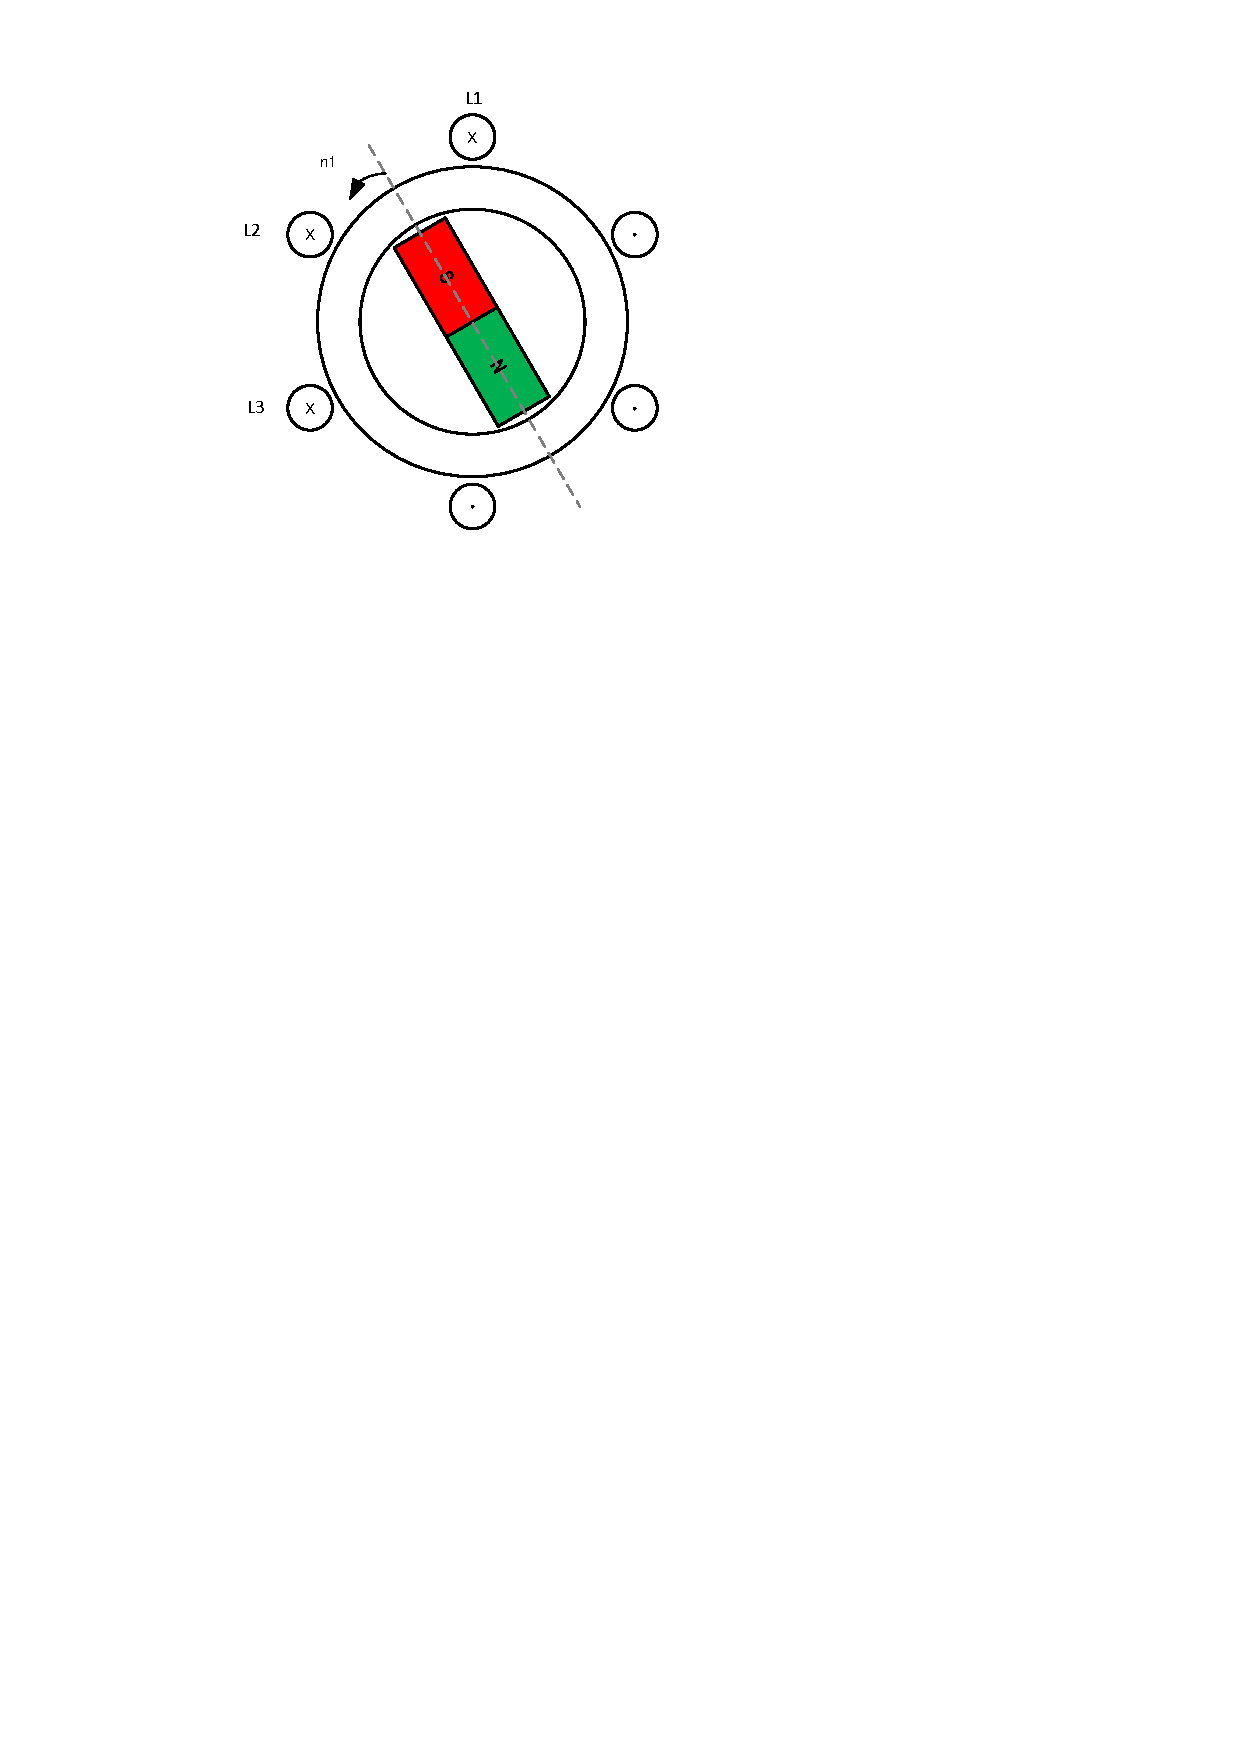
\includegraphics[width=0.5\textwidth]{Visio-synchronmaschine-drehstrom.pdf}
\label{fig:drehstromwicklung}
\caption{Erzeugung einer mehrphasigen Spannung durch ein räumlich sinusförmiges Läuferdrehfeld in Anlehnung an \autocite[S.~141]{fischer2009}}
\end{figure}

\section{Induktivitäten}\label{sec:induktiv}

\section{Einführung Synchronmaschine}\label{sec:synchron}

\paragraph{Historischer Hintergund} Die ersten Synchronmaschinen wurden als Einphasengenerator entwickelt und gebaut, den ersten dreiphasigen Synchrongenerator entwickelten 1887 unabhängig voneinander F.~A.~Haselwander\footnote{Friedrich August Haselwander war ein deutscher Ingenieur, ein Erfinder der Drehstrom-Synchronmaschine und des kompressorlosen Ölmotors.} und C.~S.~Bradley\footnote{Charles Schenk Bradley war ein US-amerikanischer Elektrotechniker, Erfinder und Pionier von frühen Elektromotoren. Er zählt neben F.~A.~Haselwander zu den Begründern des heute im Bereich der elektrischen Energietechnik eingesetzten Dreiphasenwechselstromes.} Bei den Entwicklungen bildeten sich die Bauformen der Schenkelpol- und Vollpolmaschine aus. Die Weiterentwicklung der Synchronmaschine hing stark mit dem Ausbau der Energieversorgung und dem Bedarf von leistungsstärkeren Generatoren zusammen. Unabhängig von der Entwicklung wurden schon sehr früh Synchronmaschinen als Antriebsmaschinen für eine konstante Drehzahlregelung oder einen Phasenbetrieb in der Industrie eingesetzt \autocites[S.~108f.]{ternes2012}[S.~287]{fischer2009}[S.~485f.]{mullerI2005}.

Die gleichstromgespeiste Erregerwicklung ermöglicht es, das Magnetfeld unabhängig vom Netz zu beeinflussen.
Als Spannungsquelle für die Speisung der Erregerwicklung wurden sog.\ Gleichstromerregermaschinen eingesetzt, in der heutigen Zeit werden Wechselspannung mit Hilfe von Leistungselektronischen Schaltungen gespeist.
Um die Schleifringübertragung der Erregerleistung zu umgehen, werden schleifring- bzw.\ bürstenlose Erregersysteme realisiert \autocite[S.~108]{ternes2012}.
Als Motor wurden Drephasen-Synchronmaschinen schon bald für große Leistungen eingesetzt, \zB zum Antrieb von Pumpen und Verdichten \autocite[S.~486]{mullerI2005}.
Der Nachteil ist, dass die Drehzahl durch die Netzfrequenz festgelegt ist.
Die Synchronmaschine arbeitet unabhängig von der Belastung stets mit der durch die Netzfrequenz und die ausgeführte Polpaarzahl festgelegten synchronen Drehzahl.

Heute ist es möglich mit Hilfe eines Frequenzumrichters die Drehzahl der Synchronmaschine zu steuern.
Aus diesem Grund werden größere Gleichstrommaschinen durch drehzahlvariable Synchronmaschinen abgelöst.
Im Bereich kleinerer Leistungen wird anstelle der Gleichstromerregung eine Erregung durch Permanentmagnete eingesetzt.
Dabei verliert man die Beeinflussung des Erregerzustandes über den Erregerstrom, dafür erhält man eine elektrische Maschine die keine elektrische Verbindung zum Läufer erfordert.


\subsection{Beschreibung der Synchronmaschine im dq-Koordinatensystem}

\begin{figure}[!htb]
\centering
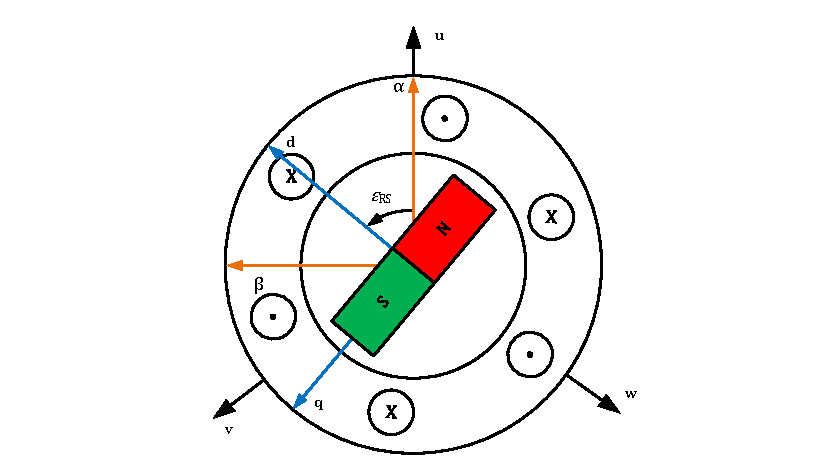
\includegraphics[width=\textwidth]{synchron-dq.pdf}
\label{fig:synchron-dq}
\caption{Darstellung der Synchronmaschine im dq-Koordinatensystem in Anlehnung an \parencite[S.~257]{schroeder2000}.}
\end{figure}

\section{Besonderheiten der Schenkelpolmaschine}\label{sec:schenkelpol}

\section{Permanenterregte Synchronmaschine}\label{sec:pmsm}

\section{Evalurierung der Ersatzschaltbilder für die Regelung}\label{sec:esb}

\begin{figure}[!htb]
\centering
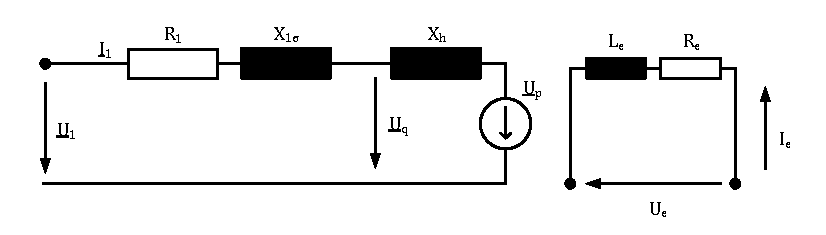
\includegraphics[width=\textwidth]{synchron-esb-kremser2004.pdf}
\label{fig:esb-kremser}
\caption{Ersatzschaltbild der Synchronmaschine nach \parencite[S.~145]{kremser2004}.}
\end{figure}

%%% Local Variables: 
%%% mode: latex
%%% TeX-master: "main"
%%% TeX-open-quote: "\\enquote{"
%%% TeX-close-quote: "}"
%%% LaTeX-csquotes-open-quote: "\\enquote{"
%%% LaTeX-csquotes-close-quote: "}"
%%% End: 


%% -*- coding: utf-8 -*-
% !TEX encoding = UTF-8 Unicode
% !TEX root =  main.tex

\chapter{XXXX}
\label{chap:XXXX}







%%% Local Variables: 
%%% mode: latex
%%% TeX-master: "main"
%%% TeX-open-quote: "\\enquote{"
%%% TeX-close-quote: "}"
%%% LaTeX-csquotes-open-quote: "\\enquote{"
%%% LaTeX-csquotes-close-quote: "}"
%%% End: 

%\input{Kapitel_3}
%\input{Kapitel_4}
%\input{Kapitel_5}
%\input{Kapitel_6}
% ----------------------------------------------------------------------------------------------------------
% Literatur
% ----------------------------------------------------------------------------------------------------------
\cleardoublepage
\nocite{*}
\printbibliography
% ----------------------------------------------------------------------------------------------------------
% Anhang
% ----------------------------------------------------------------------------------------------------------
\appendix
\chapter{Anhang}



\end{document}